\begin{exercise}{Le pont}{2}{Sup}
{Optique}{lelay}

La photographie du pont ci-dessous (hauteur spécifiée sur le panneau : 4,30 m) a été réalisée avec un appareil photo 
argentique :
\begin{itemize}
    \item Format de l’image sur la pellicule : 24 mm x 36mm
    \item Distance focale de l’objectif assimilé à une lentille mince convergente de focale : $f’$ = 35 mm
\end{itemize}

\begin{figure}[H]
    \centering
    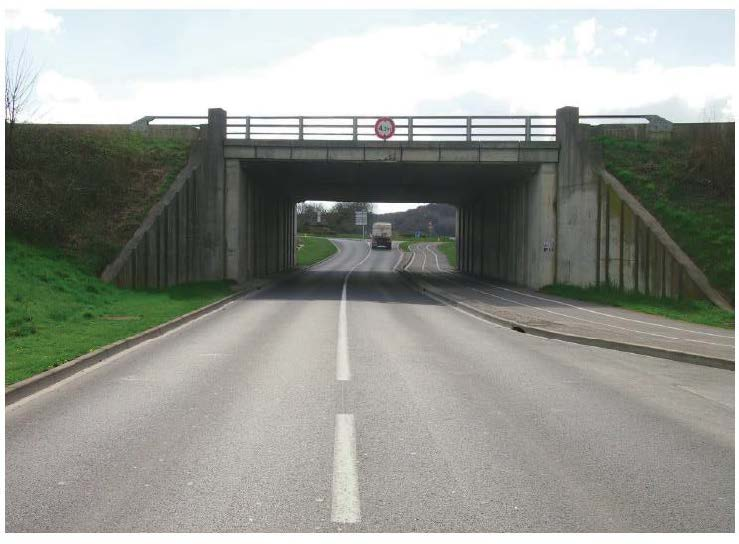
\includegraphics[width=1.\linewidth]{optique/optiquegeometrique/POOOOOOONT.jpg}
    \caption{Pont.}
\end{figure}

\begin{questions}
    \questioncours Foyers optiques, distance optique, vergence.
    \question Estimer la profondeur $p$ du pont et la distance $D$ entre l'entrée du pont et l'appareil photographique.
\end{questions}

\end{exercise}